\documentclass{report}

\usepackage{textcomp}
\usepackage{graphicx}
\usepackage{fancyhdr}
\usepackage{subcaption}
\usepackage{multicol}
\usepackage{outlines}
%===================================
\newcommand{\classinfo}{{\bf RHEL LABS \\ Week 7}\\{\it CIT 217
}\\{Chaz Davis}}
\newcommand{\semester}{BCTC \\ Spring 2020}
%===================================
\newcommand{\mysection}[1]{\section*{#1}}
\newcommand{\mysubsection}[2]{\textbf{\romannumeral #1) #2}}
%===================================
\setlength{\headheight}{15.2pt}
\pagestyle{fancy}
\fancyhf{}
\lhead{ \fancyplain{}{Chaz Davis} }
\rhead{ \fancyplain{}{\today} }
\cfoot{ \fancyplain{}{\thepage} }
\renewcommand{\headrulewidth}{0.5pt}
\renewcommand{\footrulewidth}{0pt}

%===================================
\title{\classinfo}
\author{\semester}
\date{\today}

%===================================

\begin{document}

\maketitle

%===================================
\mysection{\textbf{ Chapter 13 }}


\mysubsection{1}{Use the yum command to install Ruby. Provide the output.}


As you can see in You can see in Fig.~\ref{Ch13}~\subref{Ch13yum} 
on Pg.~\pageref{Ch13}  I entered the command 
{\scriptsize{\verb$yum install -y ruby$}\normalsize}.
You can see in You can see in Fig.~\ref{Ch13}~\subref{Ch13ruby} 
on Pg.~\pageref{Ch13} that it was successfully installed.
\hfill\break


\noindent\mysubsection{2}{Disable the rhel\_dvd yum repository and provide the output.}


I ran {\scriptsize{\verb$yum repolist$}\normalsize} to see the contents of the
repo list. I then 
ran {\scriptsize{\verb$yum-config-manager --disable rhel_dvd$}\normalsize} 
to remove it and then ran {\scriptsize{\verb$yum repolist$}\normalsize} again,
the output of which you can see in You can see in Fig.~\ref{Ch13}~\subref{Ch13dvd} 
on Pg.~\pageref{Ch13}. 
\hfill\break


\noindent\mysubsection{3}{Download wonderwidgets-1.0-4.x86\_64\.rpm from http://classroom/pub/materials/ within the NetLab environment. Using the rpm command, provide the output of the file contents.}


I ran {\scriptsize{\verb$wget wonderwidgets-1.0-4.x86_64.rpm$}\normalsize} to
download the required files. Then to show the contents I ran the command
{\scriptsize{\verb$rpm -q -p wonderwidgets-1.0-4.x86_64.rpm -l$}\normalsize} 
As you can see in Fig.~\ref{Ch13}\subref{Ch13widg} on Pg.~\pageref{Ch13}.
\hfill\break


\begin{figure}[!b]\centering
\subfloat[Yum Install]{\label{Ch13yum}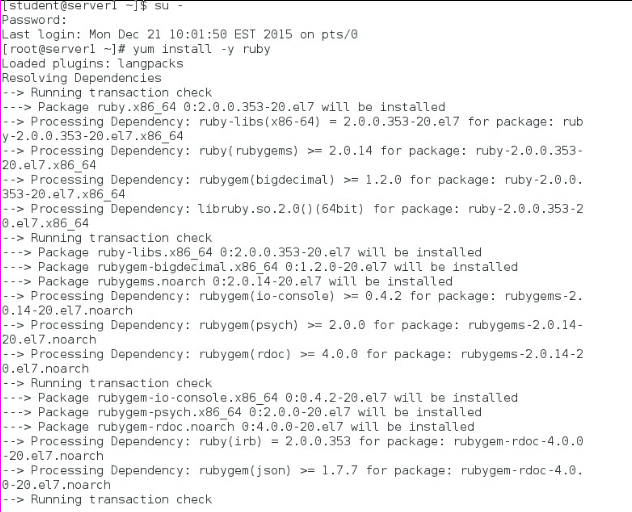
\includegraphics[width=.75\linewidth]{Figures/2020-02-29-055301_632x512_scrot.png}}\par
\subfloat[Ruby successfully installed]{\label{Ch13ruby}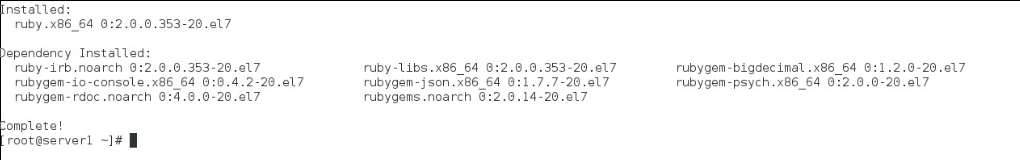
\includegraphics[width=.85\linewidth]{Figures/2020-02-29-055322_1020x160_scrot.png}}\par
\subfloat[Rhel dvd removal]{\label{Ch13dvd}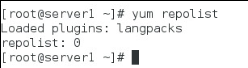
\includegraphics[width=.45\linewidth]{Figures/2020-02-29-060431_248x68_scrot.png}}\par
\subfloat[Wonderwidgets]{\label{Ch13widg}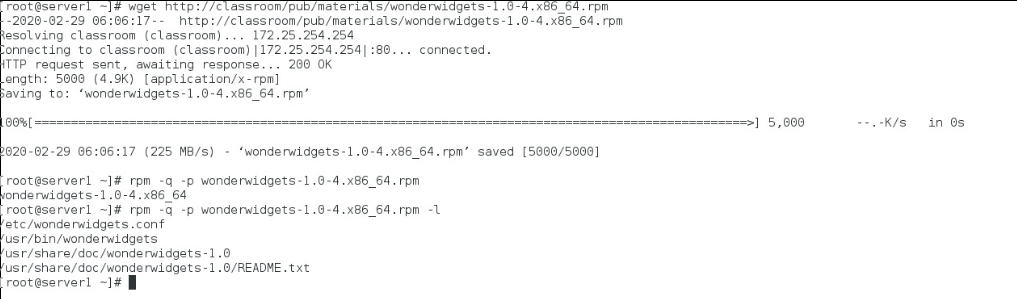
\includegraphics[width=.75\linewidth]{Figures/2020-02-29-060738_1017x299_scrot.png}}\par
\caption{Running the commands in Chapter 13 Labs}
\label{Ch13}
\end{figure}

\clearpage

%===================================
\mysection{\textbf{Chapter 14 }}


\mysubsection{1}{Make a symbolic link of the /etc/hosts in your home directory. Provide a detailed list of the files in your home directory.}
As you can see in You can see in Fig.~\ref{Ch14}~\subref{Ch14soft} 
on Pg.~\pageref{Ch14} I ran {\scriptsize{\verb$ln -s /etc/hosts /home/student$}\normalsize} 
and then ran {\scriptsize{\verb$ls -al$}\normalsize} to get the output of the
directory.

\noindent\mysubsection{2}{Find out the size, used, and available space of all mounted file systems. Provide the output in human-readable format.}


I ran the command {\scriptsize{\verb$df -h$}\normalsize} to get a human
readable output of the filesystems, as you can see in You can see in
Fig.~\ref{Ch14}~\subref{Ch14df} 
on Pg.~\pageref{Ch14}.


\noindent\mysubsection{3}{Search the filesystem for the location of the redhat-release file. Provide the output of the location.}


I ran the command {\scriptsize{\verb$locate redhat-release$}\normalsize} the
output of which you can see You can see in Fig.~\ref{Ch14}~\subref{Ch14locate} 
on Pg.~\pageref{Ch14}.



\begin{figure}[!hbt]\centering
\subfloat[Soft link to home dir]{\label{Ch14soft}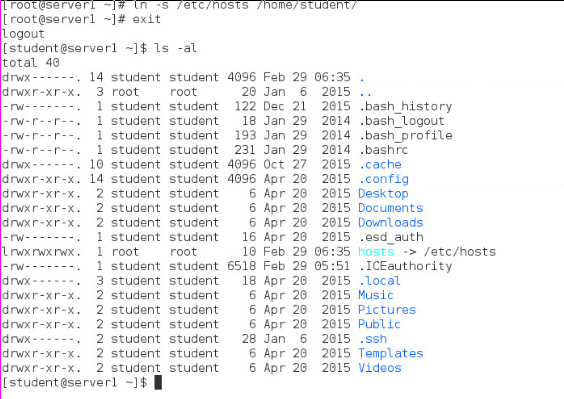
\includegraphics[width=.65\linewidth]{Figures/2020-02-29-063612_564x399_scrot.png}}\par
\subfloat[Filesystems]{\label{Ch14df}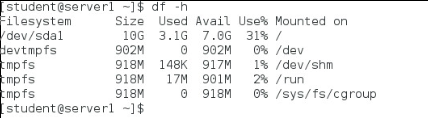
\includegraphics[width=.50\linewidth]{Figures/2020-02-29-064303_428x118_scrot.png}}\par 
\subfloat[Running the locate command]{\label{Ch14locate}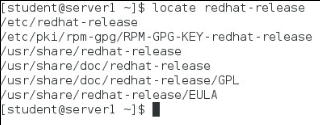
\includegraphics[width=.50\linewidth]{Figures/2020-02-29-064505_320x125_scrot.png}}
\caption{Screenshots of commands from Chapter 14}
\label{Ch14}
\end{figure}




%===================================

\end{document}
